\documentclass{include/protokollclass}
% Main File - Based on protokollclass.cls
% Comments are mostly in English (and some in German, concerning the Praktikum)
% ------------------------------------------------------------------------------
% Further files in folder:
%  - include/cmds.tex (for macros and additional commands)
%  - include/kitlogo.pdf (for titlepage)
%  - lit.bib (bibtex bibliography database)
%  - include/titlepage.tex (for layout of titelpage)
% ------------------------------------------------------------------------------
% Useful Supplied Packages:
% amsmath, amssymb, mathtools, bbm, upgreek, nicefrac,
% siunitx, varioref, booktabs, graphicx, tikz, multicol





%% ---------------------------------------------
%% |    Informationen über dieses Protokoll    |
%% ---------------------------------------------
\newcommand{\praktikum}{P1}                % P1 oder P2
\newcommand{\semester}{WS21/22}            % z.B. "WS14/15" oder "SS15"

\newcommand{\wochentag}{Do}                % Mo, Di, Mi oder Do
\newcommand{\gruppennr}{7}                % Zweistellige Gruppennummer

\newcommand{\nachnamea}{Linn}             % Nachname des ersten Praktikanten
\newcommand{\vornamea}{Myriel}               % Vorname des ersten Praktikanten
\newcommand{\nachnameb}{Schwartz}           % Nachname des zweiten Praktikanten
\newcommand{\vornameb}{Arne}              % Vorname des zweiten Praktikanten

\newcommand{\emailadressen}{uhreq@student.kit.edu, ukjfu@student.kit.ed}
% optionale Angabe von Emailadresse(n) für den Kontakt mit dem Betreuer

\newcommand{\versuch}{Lichtgeschwindigkeit} % Name des Versuchs
\newcommand{\versuchsnr}{80}               % bitte die korrekte Nummer dem 
                                           % Arbeitsplatz am Versuchstag 
                                           % entnehmen
\newcommand{\fehlerrechnung}{Ja}         % Ob Fehlerrechnung im Versuch 
                                           % durchgeführt wurde oder nicht

\newcommand{\betreuer}{Adrian Kriewitz}      % Name des zuständigen Betreuers
\newcommand{\durchgefuehrt}{18.11.21}      % Datum, an dem der Versuch 
                                           % durchgeführt wurde





%% --------------------------------------
%% |    Settings for Word Separation    |
%% --------------------------------------
% Help for separation:
% In German package the following hints are additionally available:
% "- = Additional separation
% "| = Suppress ligation and possible separation (e.g. Schaf"|fell)
% "~ = Hyphenation without separation (e.g. bergauf und "~ab)
% "= = Hyphenation with separation before and after
% "" = Separation without a hyphenation (e.g. und/""oder)

% Describe separation hints here:
\hyphenation
{
    über-nom-me-nen an-ge-ge-be-nen
    %Pro-to-koll-in-stan-zen
    %Ma-na-ge-ment  Netz-werk-ele-men-ten
    %Netz-werk Netz-werk-re-ser-vie-rung
    %Netz-werk-adap-ter Fein-ju-stier-ung
    %Da-ten-strom-spe-zi-fi-ka-tion Pa-ket-rumpf
    %Kon-troll-in-stanz
}





% um die Titelseite per PDF-reader auszufüllen. Vorgefertigte Daten
% können in Datei 'data.tex' modifiziert werden.
%\setboolean{forminput}{true}
% um die Anmerkungen zu den Textfeldern anzeigen zu lassen
%\setboolean{showannotations}{true}
% Erneuern der Seitenzahl in jedem Kapitel
%\setboolean{chapResetPageNumb}{true}
% Einbinden der Kapitelnummer in der Seitenzahl
%\setboolean{chapWiseNumb}{true}
% english or ngerman (new german für neue deutsche Rechtschreibung statt german)
\SelectLanguage{ngerman}

\usepackage{multirow}



%% -----------------------
%% |    Main Document    |
%% -----------------------
\begin{document}
    % Titlepage und ToC
    \FrontMatter

    % coordinates for background border
\newcommand{\diameter}{20}
\newcommand{\xone}{-15}
\newcommand{\xtwo}{160}
\newcommand{\yone}{15}
\newcommand{\ytwo}{-253}

\newcommand{\hoehea}{55}
\newcommand{\hoeheb}{55}




\begin{titlepage}
    % background border
    \begin{tikzpicture}[overlay]
    \draw[color=gray]  
            (\xone mm, \yone mm)
      -- (\xtwo mm, \yone mm)
    arc (90:0:\diameter pt) 
      -- (\xtwo mm + \diameter pt , \ytwo mm) 
        -- (\xone mm + \diameter pt , \ytwo mm)
    arc (270:180:\diameter pt)
        -- (\xone mm, \yone mm);
    \end{tikzpicture}
    
    % KIT logo
    \begin{textblock}{10}[0,0](4.5,2.5)
        
\includegraphics[width=.25\textwidth]{include/kitlogo.pdf}
    \end{textblock}
    \changefont{phv}{m}{n}    % helvetica
    \begin{textblock}{10}[0,0](5.5,2.2)
        \begin{flushright}
            \Large FAKULTÄT FÜR PHYSIK\\Praktikum Klassische Physik
        \end{flushright}
    \end{textblock}
    
    \begin{textblock}{10}[0,0](4.2,3.1)
        \begin{tikzpicture}[overlay]
        \draw[color=gray]
            (\xone mm + 5 mm, -8 mm)
         -- (\xtwo mm + \diameter pt - 5 mm, -8 mm);
        \end{tikzpicture}
    \end{textblock}
    
    \Large
    % Zeile 1
    \begin{textblock}{12}[0,0](3.58,4)
        \mytextfield{Prak.}{\praktikum}{0.9cm}{17pt}
                    {P1/P2}{2}{Praktikum}
    \end{textblock}
    \begin{textblock}{12}[0,0](5.53,4)
        \mytextfield{Semester}{\semester}{2.6cm}{17pt}
        {z.B. \glqq WS14/15\grqq\ oder \glqq SS15\grqq}{0}{Semester}
    \end{textblock}
    \begin{textblock}{12}[0,0](9.53,4)
        \mytextfield{Wochentag}{\wochentag}{1.3cm}{17pt}
                    {Mo/Di/Mi/Do}{2}{Wochentag}
    \end{textblock}
    \begin{textblock}{12}[0,0](12.88,4)
       \mytextfield{Gruppennr.}{\gruppennr}{1.06cm}{17pt}
                   {\#\#}{2}{Gruppennummer}
    \end{textblock}
    
    % Zeile 2
    \begin{textblock}{12}[0,0](3.58,4.55)
        \mytextfield{Name}{\nachnamea}{6cm}{17pt}
                    {}{0}{Name1}
    \end{textblock}
    \begin{textblock}{12}[0,0](9.53,4.55)
        \mytextfield{Vorname}{\vornamea}{6cm}{17pt}
                    {}{0}{Vorname1}
    \end{textblock}
    
    % Zeile 3
    \begin{textblock}{12}[0,0](3.58,5.1)
        \mytextfield{Name}{\nachnameb}{6cm}{17pt}
                    {}{0}{Name2}
    \end{textblock}
    \begin{textblock}{12}[0,0](9.53,5.1)
        \mytextfield{Vorname}{\vornameb}{6cm}{17pt}
                    {}{0}{Vorname2}
    \end{textblock}
    
    % Zeile 4
    \begin{textblock}{12}[0,0](3.64,5.65)
       \normalsize\mytextfield{Emailadresse(n)}{\emailadressen}{13.1cm}{10pt}
                              {Optional}{0}{Emailadressen}
    \end{textblock}
    
    % Zeile 5
    \begin{textblock}{12}[0,0](3.58,6.2)
        \mytextfield{Versuch}{\versuch\ (\praktikum-\versuchsnr)}{9.45cm}{14pt}
                    {z.B. \glqq Galvanometer (P1-13)\grqq\ oder \glqq %
                     Mikrowellenoptik (P2-15)\grqq}{0}{Versuch}
    \end{textblock}
    \begin{textblock}{12}[0,0](12.58,6.2)
       \mytextfield{Fehlerrech.}{\fehlerrechnung}{1.46cm}{17pt}
                   {Ja/Nein}{4}{Fehlerrechnung}
    \end{textblock}
    
    % Zeile 6
    \begin{textblock}{12}[0,0](3.58,6.75)
        \mytextfield{Betreuer}{\betreuer}{7cm}{17pt}{}{0}{Betreuer}
    \end{textblock}
    \begin{textblock}{12}[0,0](10.82,6.75)
        \mytextfield{Durchgeführt am}{\durchgefuehrt}{2.53cm}{17pt}
                    {TT.MM.JJ}{8}{Durchfuehrung}
    \end{textblock}
    
    % Querstrich
    \begin{textblock}{20}[0,0](0,7.1)\tiny\centering
        Wird vom Betreuer ausgefüllt.
    \end{textblock}
    \begin{tikzpicture}[overlay]
    \draw[color=gray]
        (\xone mm + 5 mm, -78 mm)
     -- (\xtwo mm + \diameter pt - 5 mm, -78 mm);
    \end{tikzpicture}
    
    % Zeile 1
    \begin{textblock}{12}[0,0](3.58,8)
        \myTtextfield{1. Abgabe am}{}{2.5cm}{17pt}
                     {}
    \end{textblock}
    \begin{textblock}{20}[0,0](8.3,8)
        \myTtextfield{Rückgabe am}{}{2.5cm}{17pt}
                     {}
    \end{textblock}
    
    % Block 1
    \begin{tikzpicture}[overlay]
    \draw[color=gray]  
        (\xone mm + 10 mm, -85.5 mm)
     -- (\xtwo mm + \diameter pt - 10 mm, -85.5 mm)
     -- (\xtwo mm + \diameter pt - 10 mm, -85.5 mm - \hoehea mm)
     -- (\xone mm + 10 mm, -85.5 mm - \hoehea mm)
     -- (\xone mm + 10 mm, -85.5 mm);
    \end{tikzpicture}
    
    \begin{textblock}{20}[0,0](4,8.57)
        Begründung:
    \end{textblock}
    
    % Zeile 2
    \begin{textblock}{12}[0,0](3.58,11.85)
        \myTtextfield{2. Abgabe am}{}{2.5cm}{17pt}
                     {}
    \end{textblock}
    
    % Block 2
    \begin{tikzpicture}[overlay]
    \draw[color=gray]  
        (\xone mm + 10 mm, -167 mm)
     -- (\xtwo mm + \diameter pt - 10 mm, -167 mm)
     -- (\xtwo mm + \diameter pt - 10 mm, -167 mm - \hoehea mm)
     -- (\xone mm + 10 mm, -167 mm - \hoehea mm)
     -- (\xone mm + 10 mm, -167 mm);
    \end{tikzpicture}
    \begin{textblock}{12}[0,0](4.25,12.24)
        {Ergebnis:~~~~+~~~/~~~0~~~/~~~-}
    \end{textblock}
    \begin{textblock}{12}[0,0](9.1,12.24)
        {Fehlerrechnung:~~~Ja~~~/~~~Nein}
    \end{textblock}
    \begin{textblock}{12}[0,0](4.05,12.9)
        \myTtextfield{Datum}{}{2.5cm}{17pt}
                     {}
    \end{textblock}
    \begin{textblock}{12}[0,0](8.9,12.9)
        \myTtextfield{Handzeichen}{}{5.5cm}{17pt}
                     {}
    \end{textblock}
    \begin{textblock}{12}[0,0](4,13.4)\Large
        {Bemerkungen:}
    \end{textblock}
    
    
    
    % lowest text blocks concerning the KIT
    \begin{textblock}{10}[0,0](4,16.8)
        \tiny{KIT -- Universität des Landes Baden-Württemberg und nationales %
              Forschungszentrum in der Helmholtz-Gemeinschaft}
    \end{textblock}
    \begin{textblock}{10}[0,0](14,16.75)
        \large{\textbf{www.kit.edu}}
    \end{textblock}
\end{titlepage}
 %\cleardoublepage

    \begingroup \let\clearpage\relax    % in order to avoid listoffigures and
    \tableofcontents                    % listoftables on new pages
    \listoffigures
    \listoftables
    \endgroup
    %\cleardoublepage



    % Contents
    \MainMatter
    \chapter{Drehspiegelmethode}
    \section{Vorbereitung auf den Versuch}

In diesem Versuch geht es darum, die Größe der Lichtgeschwindigkeit mithilfe der Drehspiegelmethode zu bestimmen (Abb. \ref{fig:Drehspiegelmethode}). Dafür wird ein Laserstrahl über einen Strahlenteiler geschickt, wobei dieser dahinter auf einen Drehspiegel trifft, der sich mit regulierbarer Frequenz dreht. Der Strahl durchquert eine Linse und trifft, nach einer weiteren Umlenken durch einen Spiegel, senkrecht auf einen Endspiegel. Der Strahlengang kehrt sich nun um, wobei sich der Drehspiegel in der Zwischenzeit um einen Winkel $\delta$ weitergedreht hat. Vom Strahlteiler wird dieser nun auf den Schirm geschickt.\\

\begin{figure}
    \centering
    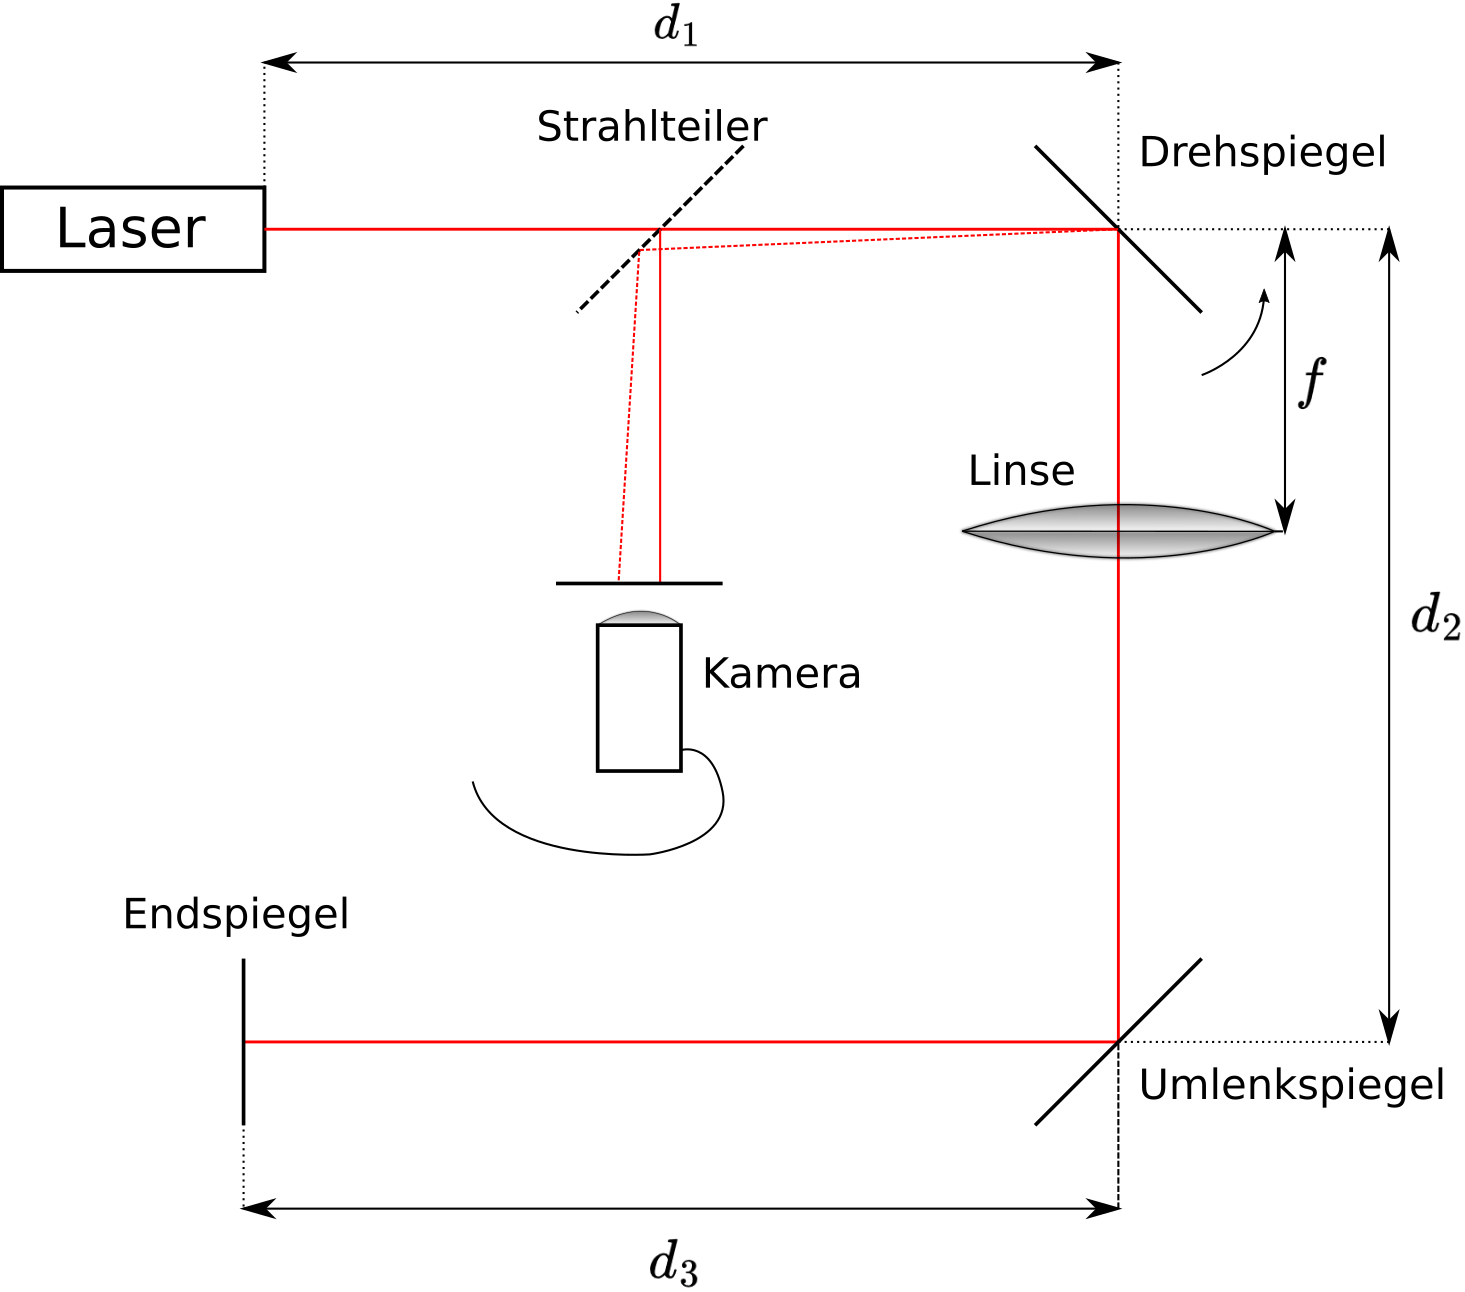
\includegraphics[scale=0.6]{Lichtgeschwindigkeit/Protokoll/fig/Drehspiegelmethode.png}
    \caption{Drehspiegelmethode}
    \label{fig:Drehspiegelmethode}
\end{figure}

Gemessen wird nun der Abstand a, also der Abstand zu dem Punkt, wo der Strahl bei ruhendem Drehspiegel auftreffen würde. Dieser wird auf der Millimeterskala auf dem Schirm für unterschiedliche Frequenzen gemessen.\\
Da der Versuch schon aufgebaut wurde, sind einige Werte, die für die Auswertung wichtig sind, schon gegeben. Diese sind in Tabelle \ref{tab:Drehspiegel vorgegebene Werte} aufgeführt.

\begin{table}[h]
    \centering
    \caption{Gegebene Werte Versuchsaufbau Drehspiegel}
    \begin{tabular}{c c c}
    \hline
    Abstand & Symbol & Wert \\
    \hline
    Laser-Drehspiegel Maximal & $d_{1max}$ & \SI{6.8}{\metre} \\
    Laser-Drehspiegel & $d_1$ & \SI{6.51}{\metre}\\
    Drehspiegel-Umlenkspiegel & $d_2$ & \SI{7.23}{\metre}\\
    Umlenkspiegel-Enspiegel & $d_3$ & \SI{6.59}{\metre}\\
    Brennweite Linse & $f$ & \SI{5}{\metre}\\
    
    \hline
    \end{tabular}
    \label{tab:Drehspiegel vorgegebene Werte}\\
    Fehler auf alle gegebenen Werte \SI{0.03}{\metre}.
\end{table}

Vorbereitend sollen nun die Positionen von Linse und Laseraustrittsöffnung berechnet werden. In diesem Versuchsaufbau wird eine Linse verwendet, damit der Strahl sowohl auf dem Dreh- als auch auf dem Enspiegel gebündelt wird und man somit ein scharfes Bild bekommt. Damit dies der Fall ist, muss der Abstand zwischen Drehspiegel und Linse gerade der Brennweite entsprechen. Um nun kann man sich die Gesetze der geometrischen Optik zu nutze machen \cite{2}. Man erhält durch Anwendung der Linsenleichung: 

\begin{equation}
    \frac{1}{f} = \frac{1}{b} + \frac{1}{g} = \frac{1}{d_1 + f} + \frac{1}{d_2 - f + d_3}
\end{equation}

Diese Formel wird nun nach $d_1$ umgestellt und man erhält:

\begin{equation}
    d_1 = \frac{f^2}{d_2+d_3-2f} \approx \SI{6.544}{\metre}
\end{equation}

Dieser Wert dient nur zur Überprüfung des voreingestellten Werts und dieser kann somit, da es nur eine kleine Abweichung gibt, übernommen werden.

Aus dem Abstand $a$ kann man nun auf die Lichtgeschwindigkeit schließen, die Formel dafür wird im folgenden hergeleitet:\\
Der Abstand a ist abhängig vom Winkel $\delta$, um den sich der Drehspiegel dreht, während das Licht den skizzierten Weg zurücklegt. Man erhält:

\begin{equation} \label{a}
    a = d_1 \tan{2\delta} \approx 2\delta d_1
\end{equation}

Man erhält nun weiter für die Zeitdifferenz $\Delta t$, die der Laserstrahl braucht:

\begin{equation}
    \Delta t = \frac{\delta}{\omega} = \frac{\delta}{2\pi f} \stackrel{(\ref{a})}{=} \frac{a}{4\pi f d_1}
\end{equation}

Und für die Streckendifferenz $\Delta s$:

\begin{equation}
    \Delta s = 2(d_2 + d_1)
\end{equation}

Der Wert für die Lichtgeschwindigkeit ergibt sich nun aus der Differenz von $\Delta s$ und $\Delta t$:

\begin{equation} \label{Drehspiegelmethode Formel}
    c = \frac{\Delta s}{\delta t} = \frac{8\pi f d_1 ( d_2 + d_3)}{a}
    \Rightarrow a = \frac{8 \pi f d_1 (d_2 + d_3)}{c}
\end{equation}

Es soll zusätzlich noch der erwartete Effekt berechnet werden, dafür werden die gegebenen Werte, zusammen mit dem Literaturwert für die Lichtgeschwindigkeit $c$ und einer Frequenz von $f = \SI{500}{\Hz}$ in die Formel \ref{Drehspiegelmethode Formel} eingesetzt und man erhält $a \approx \SI{0.00377}{\metre} = \SI{3.77}{\milli\metre}$.

\section{Justierung der Apparatur und Messung}

Die Justierung und das überprüfen der Positionen der Spiegel und der anderen Objekte enfiel, da der Versuch schon fertig aufgebaut vorgefunden wurde. Bei der Durchführung der Messungen wurde die Ablenkung a in Abhängigkeit von der Rotationsfrequenz des Drehspiegels notiert. Die Messwerte sind in Tabelle \ref{tab:Messwerte Drehspiegelmethode} aufgetragen.

\begin{table}[h]
    \centering
    \caption{Messwerte Drehspiegelmethode}
    \label{tab:Messwerte Drehspiegelmethode}
    \begin{tabular}{c c}
    \hline
    Rotationsgeschwindigkeit in $\frac{U}{m}$ & Lasserstrahlauftreffposition in $mm$ \\
    \hline
    1000 & 24.4 \\
    2000 & 24.5 \\
    3000 & 24.6 \\
    3950 & 24.7  \\
    4950 & 24.9 \\
    6000 & 25 \\
    6900 & 25.1\\
    8000 & 25.2 \\
    9050 & 25.3 \\
    10000 & 25.4 \\
    11000 & 25.4 \\
    12020 & 25.6 \\
    12970 & 25.9 \\
    13950 & 26 \\
    15000 & 26.1 \\
    \hline
    \end{tabular}
\end{table}

\section{Auswertung}

Die Formel \ref{Drehspiegelmethode Formel} lässt sich so umschreiben, dass man direkt die Drehzahl des Rotationsspiegels U einsetzen kann: 

\begin{equation} \label{Drehspiegelmethode Formel Drehzahl}
    a = \frac{8 \pi  d_1 (d_2 + d_3)}{60c} U
\end{equation}

Mit dieser Formel und den Messdaten aus Tabelle \ref{tab:Messwerte Drehspiegelmethode} wird nun eine lineare Regression durchgeführt (Abb. \ref{fig:Drehspiegelmethode Anpassung} )

Für die Steigung ergibt sich somit: 
\begin{equation} \label{Steigung Drehspiegelmethode}
    m = \frac{8 \pi  d_1 (d_2 + d_3)}{60c} = 8290 \, \frac{1}{mm\cdot s}
\end{equation}

Durch Umformung der Gleichung \ref{Drehspiegelmethode Formel Drehzahl} und einsetzen von m erhält man:

\begin{equation}
    c = m \frac{8 \pi d_1 (d_2+d_2)}{60}  \stackrel{(\ref{Steigung Drehspiegelmethode})}{\Rightarrow} c = \SI{287940287.054}{\metre\per\second}
\end{equation}

\begin{figure}[ht]
    \centering
    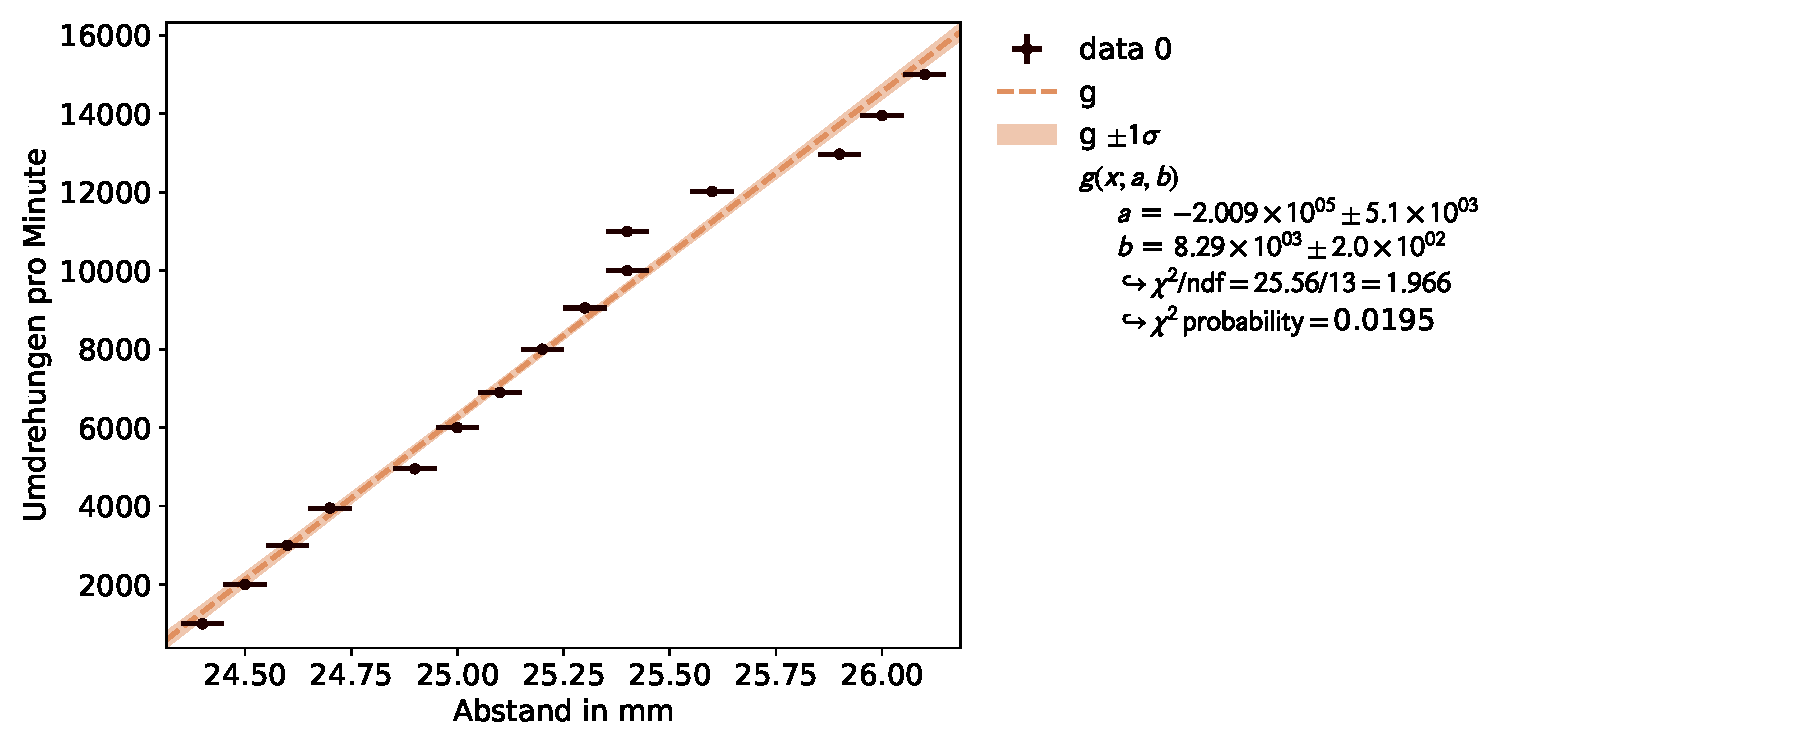
\includegraphics[scale=0.45]{Lichtgeschwindigkeit/Protokoll/fig/Drehspiegelmethode.pdf}
    \caption{Lineare Regression Drehspiegelmethode}
    \label{fig:Drehspiegelmethode Anpassung}
\end{figure}

\section{Fehlerrechnung}

\subsection{Statistischer Fehler}

Den statistischen Fehler entnehmen wir dem Plot. Somit erhält man einen von Kafe2 bestimmten Fehler auf die Steigung von $\pm 200 \, \frac{1}{mm \cdot s}$. Den statistischen Fehler auf die berechnete Lichtgeschwindigkeit erhält man nun durch die Gaußsche Fehlerfortpflanzung:

\begin{equation}
    \sigma_{c_{stat}} = \sqrt{(\frac{\partial c }{\partial m})^2 \sigma_m^2} = \sqrt{( \frac{8 \pi d_1 (d_2+d_2)}{60})^2 \sigma_m^2} \approx \SI{7706226}{\metre\per\second}
\end{equation}

Wie man erkennen kann, ist die statistische Abweichung größer als die Abweichung zum Literaturwert. Also müssen auch die systematischen eine signifikante Rollte spielen. 

\subsection{Systematischer Fehler}

Mögliche Fehlerquellen sind zum Beispiel:
\begin{itemize}
    \item Skala zum Ablesen der Laserpunktposition
    \item Bestimmung der Positionen der Spiegel und anderer Objekte
    \item Frequenzbestimmung des Drehspiegels
\end{itemize}

Zur Berechnung des systematischen Fehlers wird die Formel für die Größtfehlerabschätzung verwendet. Für die Lichtgeschwindigkeit gilt nach Gleichung \ref{Drehspiegelmethode Formel Drehzahl}:

\begin{equation}
    c = \frac{8 \pi  d_1 (d_2 + d_3)}{60a} U
\end{equation}

Damit ergibt sich für die Größtfehlerabschätzung:

\begin{align}
    \Delta_c &= \Bigl| \frac{\partial c}{\partial U} \Bigl| \Delta_U + \Bigl|
    \frac{\partial c}{\partial d_1} \Bigl| \Delta_{d_1} + \Bigl| \frac{\partial
    c}{\partial d_2} \Bigl| \Delta_{d_2} + \Bigl| \frac{\partial c}{\partial d_3}
    \Bigl| \Delta_{d_3} + \Bigl| \frac{\partial c}{\partial a} \Bigl| \Delta_a \\
    \Delta_c &= 8 \pi d_1 \frac{d_2 + d_3}{60a}\Delta U + 8 \pi U \frac{d_2 + d_3}{60a}\Delta d_1 + 8 \pi U d_1 \frac{1}{60a} \Delta d_2 + 8 \pi U d_1 \frac{1}{60a} \Delta d_3 + 8 \pi U d_1 \frac{d_2 + d_3 }{60a^2} \Delta a \\
    \Delta_c &= \SI{4030775.874}{\metre\per\second}
\end{align}

\subsection{Messergebnis}

Mithilfe der berechneten Werte, kann man nun das Messergebnis angeben:

\begin{align}
    c_{ges} &= c \pm \sigma_c \pm \Delta_c \\
    c_{ges} &= \SI{287940287.054}{\metre\per\second} \pm \SI{7706226}{\metre\per\second} \pm  \SI{4030775.874}{\metre\per\second}\\
    c_{ges} &= \SI{287940287.054 \pm 11737001.87}{\metre\per\second} \\
     c_{ges} &= \SI{287940287.054}{\metre\per\second} \pm 4.07 \%
\end{align}

Der Literaturwert beläuft sich auf $c_0 = 2.998 \cdot 10^8 \, \frac{m}{s}$, somit liegt der Literaturwert innerhalb unserer Fehlergrenzen.
Ein zufriedenstellendes Ergebnis
    \chapter{Phasenvergleichsmethode}
    \section{Aufbau und Durchführung}

Bei dieser Versuchsreihe wird die Lichtgeschwindigkeit über die Zeitdifferenz zwischen dem Senden und dem Empfangen von Lichtimpulsen errechnet.
Die gemessen wird die Zeitdifferenz in Abgängigkeit von der Entfernung zwischen Sender und Empfänger.
Der Aufbau besteht aus einer Metallschiene, auf der eine horizontal verschiebbare, rote LED Lampe angebracht ist.
An einem Ende der Schiene steht ein Oszilloskop mit einem Lichtempfänger, auf den die LED gerichtet ist.
Das Oszilloskop ist an einen Computer angeschlossen, die Messung des Phasenversatzes geschieht dann via Software.
Zusätzlich ist an dem Halter der LED ein Lasermessgerät angebracht, an dem der Abstand zwischen Lampe und Oszilloskop abgelesen wird.

Bei der Durchführung wurde die LED in verschiedene Abstände zum Oszilloskop geschoben und dann in der Software die zeitliche Verschiebung zwischen Sender (LED) und Lichtempfänger bestimmt.
Der Versuch wurde mit drei verschiedenen Medien zwischen LED und Oszilloskop durchgeführt: Luft, Wasser und Plexiglasstangen in zwei signifikant verschiedenen Längen

Aufgrund der technischen Einschränkungen des Oszilloskopes ist für diesen Versuch noch der Vergrößerungfaktor der Zeit zu berücksichtigen.
Dieser ergibt sich aus den in der Aufgabenstellungen angebenen Werten von $\omega = 2 \cdot \pi \cdot \SI{60}{MHz}$ und $\Omega = 2 \cdot \pi \cdot \SI{59,9}{MHz}$ zu:

\begin{equation}
    V = \frac{\omega}{\omega - \Omega} = \frac{\SI{60}{MHz}}{\SI{100}{KHz}} = \SI{600}{}
\end{equation}

\section{Justierung und Eichung}

Die Justierung und Eichung des Versuchsaufbaus wurde im Rahmen des Versuches nach Vorgabe des Betreuers nicht durchgeführt.

\section{Messung der Lichtgeschwindigkeit in Luft}

Der Versuch wird zunächst ohne spezielles Medium, einfach nur in Luft durchgeführt.

Es ergeben sich folgende Messwerte:

\begin{table}[h!]
    \begin{center}
        \caption{Messungen der Phasenverschiebung für verschiedene Abstände in Luft}
        \begin{tabular}{cc}
            \hline
            Abstand in $\SI{}{cm}$ & Zeitdifferenz in $\SI{}{\mu s}$ \\
            \hline
            $\SI{260,1}{}$    & $\SI{4,831}{}$ \\
            $\SI{239,3}{}$    & $\SI{4,399}{}$ \\
            $\SI{220,6}{}$    & $\SI{4,008}{}$ \\
            $\SI{200,7}{}$    & $\SI{3,643}{}$ \\
            $\SI{181,3}{}$    & $\SI{3,261}{}$ \\
            $\SI{160,0}{}$    & $\SI{2,837}{}$ \\
            $\SI{140,5}{}$    & $\SI{2,430}{}$ \\
            $\SI{119,9}{}$    & $\SI{2,040}{}$ \\
            $\SI{101,4}{}$    & $\SI{1,682}{}$ \\
            $\SI{80,8}{}$     & $\SI{1,275}{}$ \\
            $\SI{61,1}{}$     & $\SI{0,9255}{}$ \\
            $\SI{40,2}{}$     & $\SI{0,4779}{}$ \\
            $\SI{20,7}{}$     & $\SI{0,1041}{}$ \\
            \hline
            \label{tab:Messwerte-Zeitdiffernz-Abstand}
        \end{tabular}
    \end{center}
\end{table}

Die Messreihe wird 

\section{Bestimmung der Brechzahl in Wasser und Plexiglas}

Bei dieser Messung werden unterschiedliche Medien zwischen Sender und Empfänger gestellt und jeweils eine Messung ohne und mit Medium beim gleichen Abstand betrachtet, wobei die Lichtgeschwindigkeit in Luft hier mit der Lichtgeschwindigkeit im Vakuum gleichgesetzt wird.

Um die Brechzahl zu errechnen, muss man zunächst die Differenz der Zeiten aus den Messungen mit und ohne Material bilden:

\begin{equation}
    t_o' = \frac{s_l}{c_l}\,.
\end{equation}

\begin{equation}
    t_m' = \frac{s_l - s_m}{c_l} + \frac{s_m}{c_m}\,.
\end{equation}

\begin{equation}
   => t_m' - t_o' = \frac{s_m}{c_m} - \frac{s_m}{c_l}\,.
\end{equation}

Nun muss man noch die Vergrößerung berücksichtigen:

\begin{equation}
    \frac{1}{\SI{600}{} \cdot s_m} \cdot (t_m - t_o) = \frac{1}{c_m} - \frac{1}{c_l}\,.
\end{equation}

Und erhält nach Umformung:

\begin{equation}
    n_m = \frac{c_l}{c_m} = \frac{c_l}{c_m} = \frac{(t_m - t_o) \cdot c_l}{\SI{600}{} \cdot s_m} + 1\,.
\end{equation}

\subsection{Wasser}

\begin{table}[h!]
    \begin{center}
        \caption{Messungen der Phasenverschiebung für verschiedene Abstände mit Wasser, 1m}
        \begin{tabular}{cc}
            \hline
            Abstand in $\SI{}{cm}$ & Zeitdifferenz in $\SI{}{\mu s}$ \\
            \hline
            $\SI{260,1}{}$    & $\SI{5,562}{}$ \\
            $\SI{239,5}{}$    & $\SI{5,146}{}$ \\
            $\SI{219,9}{}$    & $\SI{4,739}{}$ \\
            $\SI{199,2}{}$    & $\SI{4,324}{}$ \\
            $\SI{180,6}{}$    & $\SI{3,950}{}$ \\
            $\SI{160,7}{}$    & $\SI{3,576}{}$ \\
            $\SI{139,7}{}$    & $\SI{3,136}{}$ \\
            $\SI{119,8}{}$    & $\SI{2,762}{}$ \\
            \hline
            \label{tab:Messwerte-Zeitdiffernz-Abstand-Wasser}
        \end{tabular}
    \end{center}
\end{table}

\begin{table}[H]
    \begin{center}
        \caption{Berechnete Brechzahlen für verschiedene Materialien}
        \begin{tabular}{cccc}
            \hline
            Messung            & Plexiglas ($\SI{30}{cm}$) & Plexiglas ($\SI{8}{cm}$)  \\
            \hline
            1. Messung         & $\SI{1,515}{}$            & $\SI{1,379}{}$ \\
            2. Messung         & $\SI{1,488}{}$            & $\SI{1,271}{}$ \\
            3. Messung         & $\SI{1,529}{}$            & $\SI{1,327}{}$ \\
            4. Messung         & $\SI{1,515}{}$            & $\SI{1,379}{}$ \\
            5. Messung         & $\SI{1,488}{}$            & $\SI{1,271}{}$ \\
            6. Messung         & $\SI{1,529}{}$            & $\SI{1,327}{}$ \\
            7. Messung         & $\SI{1,515}{}$            & $\SI{1,379}{}$ \\
            8. Messung         & $\SI{1,488}{}$            & $\SI{1,271}{}$ \\
            \hline
            Mittelwert         & $\SI{1,35}{}$        & \multicolumn{2}{c}{\SI{1,41}{}} \\
            Standardabweichung & $\SI{0,015}{}$       & \multicolumn{2}{c}{\SI{0,09}{}} \\
            \hline
            \label{tab:Ergebnisse-Brechzahlen}
        \end{tabular}
    \end{center}
\end{table}


\subsection{Plexiglas}

\begin{table}[h!]
    \begin{center}
        \caption{Messungen der Phasenverschiebung für verschiedene Abstände mit kurzem Plexiglasstab, 8cm}
        \begin{tabular}{cc}
            \hline
            Abstand in $\SI{}{cm}$ & Zeitdifferenz in $\SI{}{\mu s}$ \\
            \hline
            $\SI{159,3}{}$    & $\SI{2,881}{}$ \\
            $\SI{140,0}{}$    & $\SI{2,508}{}$ \\
            $\SI{119,9}{}$    & $\SI{2,161}{}$ \\
            $\SI{100,3}{}$    & $\SI{1,772}{}$ \\
            $\SI{80,3}{}$     & $\SI{1,374}{}$ \\
            $\SI{60,6}{}$     & $\SI{9,672}{}$ \\
            $\SI{40,2}{}$     & $\SI{5,776}{}$ \\
            $\SI{20,2}{}$     & $\SI{1,872}{}$ \\
            \hline
            \label{tab:Messwerte-Zeitdiffernz-Abstand-Plexi-kurz}
        \end{tabular}
    \end{center}
\end{table}

\begin{table}[h!]
    \begin{center}
        \caption{Messungen der Phasenverschiebung für verschiedene Abstände mit langem Plexiglas Stab, 30cm}
        \begin{tabular}{cc}
            \hline
            Abstand in $\SI{}{cm}$ & Zeitdifferenz in $\SI{}{\mu s}$ \\
            \hline
            $\SI{180,5}{}$    & $\SI{3,55}{}$ \\
            $\SI{160,4}{}$    & $\SI{3,135}{}$ \\
            $\SI{139,5}{}$    & $\SI{2,762}{}$ \\
            $\SI{119,7}{}$    & $\SI{2,348}{}$ \\
            $\SI{99,2}{}$     & $\SI{1,941}{}$ \\
            $\SI{80,4}{}$     & $\SI{1,602}{}$ \\
            $\SI{60,0}{}$     & $\SI{1,196}{}$ \\
            $\SI{40,8}{}$     & $\SI{0,8063}{}$ \\
            \hline
            \label{tab:Messwerte-Zeitdiffernz-Abstand-Plexi-lang}
        \end{tabular}
    \end{center}
\end{table}

\begin{table}[H]
    \begin{center}
        \caption{Berechnete Brechzahlen für Plexiglas}
        \begin{tabular}{cccc}
            \hline
            Messung            & Plexiglas ($\SI{8}{cm}$) & Plexiglas ($\SI{30}{cm}$)  \\
            \hline
            1. Messung         & $\SI{1,515}{}$            & $\SI{1,379}{}$ \\
            2. Messung         & $\SI{1,488}{}$            & $\SI{1,271}{}$ \\
            3. Messung         & $\SI{1,529}{}$            & $\SI{1,327}{}$ \\
            4. Messung         & $\SI{1,515}{}$            & $\SI{1,379}{}$ \\
            5. Messung         & $\SI{1,488}{}$            & $\SI{1,271}{}$ \\
            6. Messung         & $\SI{1,529}{}$            & $\SI{1,327}{}$ \\
            7. Messung         & $\SI{1,515}{}$            & $\SI{1,379}{}$ \\
            8. Messung         & $\SI{1,488}{}$            & $\SI{1,271}{}$ \\
            \hline
            Mittelwert         & $\SI{1,35}{}$        & \multicolumn{2}{c}{\SI{1,41}{}} \\
            Standardabweichung & $\SI{0,015}{}$       & \multicolumn{2}{c}{\SI{0,09}{}} \\
            \hline
            \label{tab:Ergebnisse-Brechzahlen}
        \end{tabular}
    \end{center}
\end{table}

\section{Bestimmung der Brechzahl mittels Lissajous-Figuren}
    \chapter{Brechzahlbestimmung mit modernem Laserentfernungsmesser}
    In diesem Versuch geht es darum mithilfe eines Laserentfernungsmessers die Brechzahl von zwei transparenten, nicht-diffusen Materialien zu bestimmen. Das ist möglich, da der Laserentfernungsmesser, die Lichtgeschwindigkeit als konstant annimmt. Dadurch zeigt das Gerät eine größere Distanz an, als es tatsächlich der Fall ist, wenn sich der Laserstrahl durch Materialien mit höherer Brechzahl als eins ausbreitet, mit dieser Tatsache lässt sich nun die Brechzahl bestimmen. Für die Brechzahlen gilt folgender Zusammenhang:

\begin{equation}
    n = \frac{c_{Vakuum}}{c_{Material}}
\end{equation}

Wir nehmen in diesem Versuch der Einfachheit halber an, dass gilt:

\begin{equation}
    n_{Luft} = 1.000272 \approx 1 = n_{Vakuum} \Rightarrow n_{Luft} \approx n_{Vakuum}
\end{equation}

Der Versuchsaufbau ist in Abbildung \ref{fig:Laserentfernungsmesser} skizziert. Die Ergebnisse der Messungen sind in Tabelle \ref{tab:Messwerte Versuch 3 Lichtgeschwindigkeit} aufgetragen.

\begin{figure}[h]
    \centering
    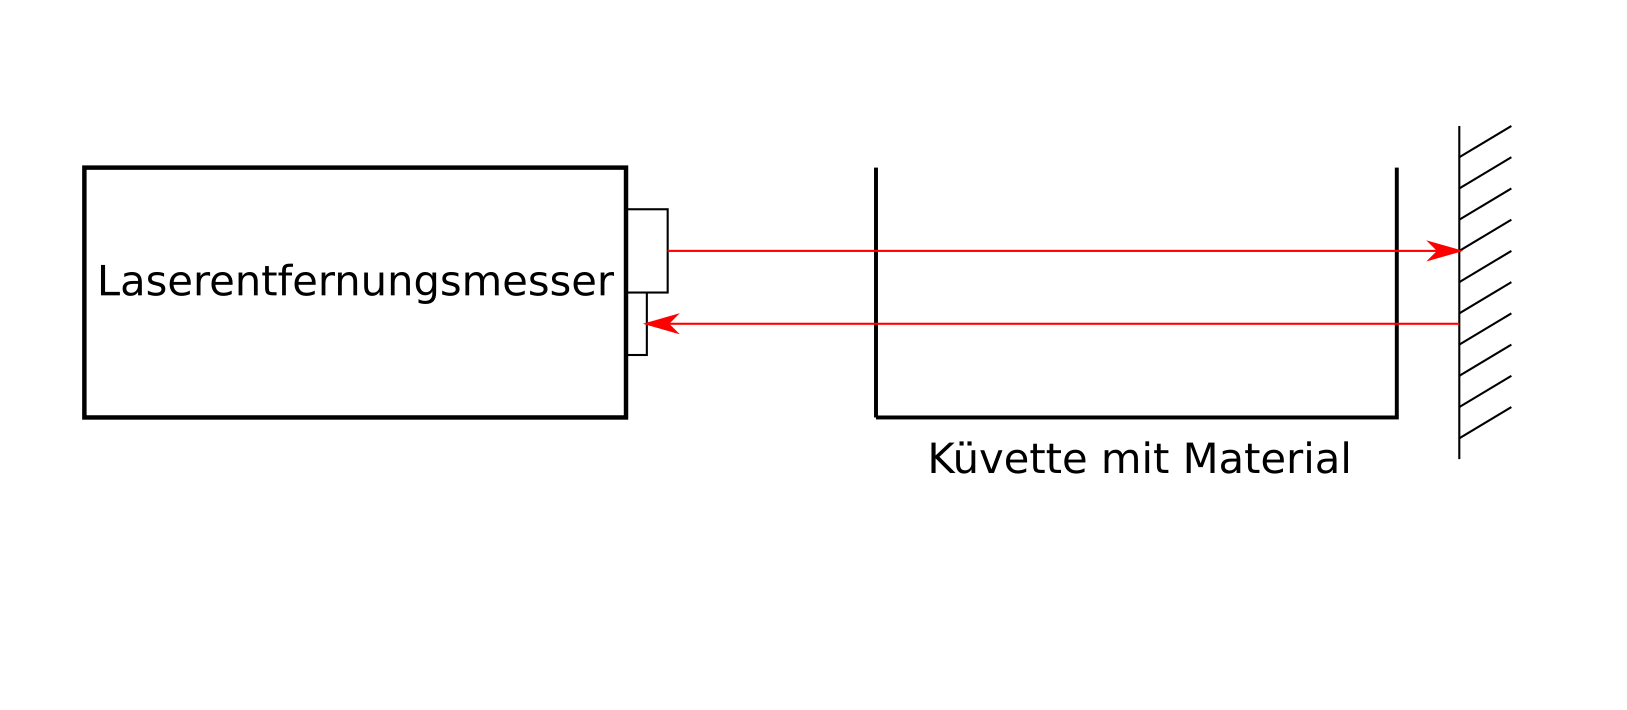
\includegraphics[scale=0.6]{./fig/Laserentfernungsmesser.png}
    \caption{Versuchaufbau für die Brechzahlbestimmung mit modernem Laserentfernungsmesser}
    \label{fig:Laserentfernungsmesser}
\end{figure}

\begin{table}
    \centering
    \caption{Messwerte für die Brechzahlbestimmung mit modernem Laserentfernungsmesser (Mittelwerte)}
    \begin{tabular}{c c c}
    \hline
    Material & Abstand in mm (quer) & Abstand in mm (längs) \\
    \hline
    Nichts & 351 & 351 \\
    Leere Küvette & - & 358.75 \\
    Silikonöl & 377 & 396.25 \\
    Wasser & 374.25 & 390.25 \\
    \hline
    \end{tabular}
    \label{tab:Messwerte Versuch 3 Lichtgeschwindigkeit}
\end{table}

Es gilt allgemein:

\begin{equation}
    t_i = \frac{s_i}{c_i} 
\end{equation}

Die Indizes geben dabei das Material an und "0" \, für die Messung mit leerer und "Gerät" \, für die Messung mit Material in der Küvette. Es folgt für die Zeit für die leere Küvette:

\begin{equation} \label{Gleichung t leer}
    t_{0} = \frac{s_{Luft} - s_{Glas}}{c_{Luft}} + \frac{s_{Glas}}{c_{Glas}} = \frac{s_{Luft}}{c_{Luft}} - \frac{s_{Glas}}{c_{Luft}} + \frac{s_{Glas}}{c_{Glas}}
\end{equation}

Daraus folgt für die Zeit für die Küvette mit Material: 

\begin{equation} \label{Gleichung t Mat}
    t_{\text{Gerät}} = \frac{s_{Luft} -s_{Glas} -s_{Mat}}{c_{Luft}} + \frac{s_{Glas}}{c_{Glas}} + \frac{s_{Luft}}{c_{Luft}} = \frac{s_{Luft}}{c_{Luft}} - \frac{s_{Glas}}{c_{Luft}} - \frac{s_{Mat}}{c_{Luft}} + \frac{s_{Glas}}{c_{Glas}} + \frac{s_{Mat}}{c_{Mat}}
\end{equation}

Damit folgt für die Differenz aus Gleichung \ref{Gleichung t leer} und \ref{Gleichung t Mat}

\begin{equation}
    t_{\text{Gerät}} - t_{0} = \frac{s_{Mat}}{c_{Mat}} - \frac{s_{Mat}}{c_{Luft}} = \frac{s_{\text{Gerät}}}{c_{\text{Gerät}}} - \frac{s_0}{s_0}
\end{equation}

Daraus folgt:

\begin{align}
    s_{\text{Gerät}} - s_0 &= s_{Mat} (\frac{c_{Luft}}{c_{Mat}} - 1) \\
    \Rightarrow n &= \frac{c_{Luft}}{c_{Mat}} = \frac{s_{\text{Gerät}} - s_0}{s_{Mat}} + 1
\end{align}

Es folgt durch einsetzen für die Brechzahlen von Wasser und Silikonöl:

\begin{table}[h]
    \caption{Brechzahlen ermittelt mit modernem Laserentfernungsmesser}
    \label{tab:Brechzahlen Laser}
    \centering
    \begin{tabular}{c c c c c}
    \hline
    Material & Brechzahl (quer) & Brechzahl (längs) & Mittelwert & Literaturwert\\
    \hline
    Silikonöl & 1.365 & 1.375 & 1.370 & 1.4 \\
    Wasser & 1.310 & 1.315 & 1.313 & 1.33 \\
    \hline
    \end{tabular}
    Quelle Literaturwerte: \url{https://www.microscope.healthcare.nikon.com/de_EU/products/optics/silicone-immersion-series}
\end{table}

 Wie man an den erhaltenen Werte gut erkennen kann, sind diese für das gewählte Messverfahren relativ genau. Für die Brechzahl von Silikonöl erhalten wir eine Abweichung von nur ca. 3\% und für die Brechzahl von Wasser von nur ca. 1\% zum Literaturwert. Was auch an den Werten zu erkennen ist, ist, dass der Wert für die Messung mit längs zum Laser orientierten Kürvette näher am Literaturwert liegt. Was daran liegt, dass das Verhältnis von Strecke im Material zur Strecke in Luft größer ist, was zu einem genaueren Wert führt.
 
 Mögliche Fehlerquellen sind: 
 
 \begin{itemize}
     \item Eichung des Laserentfernungsmessers
     \item Genauigkeit des Laserentfernungsmessers (Genauigkeit $\pm \SI{1.5}{\milli\metre}$)
     \item Reflexion an der Glaswand der Küvette, anstatt am Ende der Strecke
     \item Verschmutzungen an der Wand der Küvette oder im Material
 \end{itemize}
 
 Angesichts der Messmethode und deren Ungenauigkeit ist das Ergebnis aber zufriedenstellend.
    
    %\emptychapter[1]{Messprotokoll 1}{} % usage: \emptychapter[page displayed 
                                        %        in toc]{name of the chapter}
    %\pseudochapter[3]{Messprotokoll 2}  % usage: \pseudochapter[number of pages 
                                        %        added]{name of the chapter}
    
    %\chapter{Auswertung}
    %Ganz tolle Auswertung des Versuchs. \cite{Dem10} %\cleardoublepage

    % appendix for more or less interesting calculations
    %\Appendix
    %\chapter*{\appendixname} \addcontentsline{toc}{chapter}{\appendixname}
    % to make the appendix appear in ToC without number. \appendixname = 
    % Appendix or Anhang (depending on chosen language)
    %\section{Erster Abschnitt des Anhangs}
Dies ist der erste ganz tolle Abschnitt des Anhangs. %\cleardoublepage



    % Bibliography
    \TheBibliography

    % BIBTEX
    % use if you want citations to appear even if they are not referenced to: 
    % \nocite{*} or maybe \nocite{Kon64,And59} for specific entries
    %\nocite{*}
    %\bibliographystyle{babalpha}
    %\bibliography{lit.bib}

    % THEBIBLIOGRAPHY
    \begin{thebibliography}{000}
       \bibitem{1} Vorbereitungsmappe Lichtgeschwindigkeit
       \bibitem{2} Vorbereitungsmappe Geometrische Optik
    \end{thebibliography}
\end{document}
